\providecommand{\Cart}{\mathcal{C}art}
\providecommand{\coCart}{\mathrm{co}\mathcal{C}\mathit{art}}   %
\providecommand{\Fib}{\mathcal{F}ib}
\providecommand{\Fun}{\operatorname{Fun}}
\providecommand{\dashdownarrow}{\rotatebox[origin=c]{270}{$\dashrightarrow$}}   %

\section{双侧纤维化的∞-宇宙}\label{sec:two-sided-fibration-cosmos}

定理 7.1.4 与命题 7.1.7 的第一对等价条件，借助命题 6.3.14 的诸\trInfinityCosmos{}，%
为定义\trTwoSidedFibration{}的\trInfinityCosmos{}提供了两种等价的途径。

\begin{definition}[双侧纤维化的∞-宇宙]\label{def:two-sided-fibration-cosmos}
由定理 7.1.4 与命题 7.1.7，对\trInfinityCosmos{} $\mathcal{K}$ 中的任何一对%
\trInfinityCategory{} $A$ 与 $B$，$\mathcal{K}_{/A\times B}$ 的如下这对以%
\trQuasiCategory{}富集的子范畴
\begin{equation*}
\Cart(\coCart(\mathcal{K})_{/A})_{/\pi\colon A\times B\to A}
\qquad\text{与}\qquad
\coCart(\Cart(\mathcal{K})_{/B})_{/\pi\colon A\times B\to B}
\end{equation*}
相重合。我们记
\begin{equation*}
{}_{A\backslash}\Fib(\mathcal{K})_{/B}\subset\mathcal{K}_{/A\times B}
\end{equation*}
表示这一公共子范畴，并称之为从 $A$ 到 $B$ 的\textbf{\trTwoSidedFibration{}的%
\trInfinityCosmos}，如此称谓的理由稍后即明。

根据定义，从 $A\xleftarrow{q}E\xrightarrow{p}B$ 到
$A\xleftarrow{s}F\xrightarrow{r}B$ 的\trFunctorSpace
\begin{equation*}
\Fun_{{}_{A\backslash}\Fib(\mathcal{K})_{/B}}(E,F)
:=\Fun^{\mathrm{cart}}_{A\times B}(E,F)\subset\Fun_{A\times B}(E,F)
\end{equation*}
是由那些定义从 $E$ 到 $F$ 的\trCartesianFunctor{}的\trSpan{}映射构成的\trQuasiCategory%
（见命题 7.1.7）。

由于从 $A$ 到 $B$ 的\trTwoSidedIsofibration{}不过是 $A\times B$ 上的一个\trIsofibration{}，%
我们可以把 $\mathcal{K}_{/A\times B}$ 称作从 $A$ 到 $B$ 的\textbf{\trTwoSidedIsofibration{}的%
\trInfinityCosmos}。
\end{definition}

\begin{proposition}\label{prop:two-sided-fibration-cosmos-embedded}
对\trInfinityCosmos{} $\mathcal{K}$ 中的任何\trInfinityCategory{} $A$ 与
$B$，双侧\trFibration{}的\trInfinityCosmos{}
\[
{}_{A\backslash}\Fib(\mathcal{K})_{/B}\hookrightarrow\mathcal{K}_{/A\times B}
\]
在\trIsofibration{}的\trInfinityCosmos{}中是\trCosmologicallyEmbedded{}，
并由包含创生一个∞-宇宙结构。
\end{proposition}

\begin{proof}
该包含分解为
\begin{equation*}
\begin{array}{ccccc}
{}_{A\backslash}\Fib(\mathcal{K})_{/B} & & & & \mathcal{K}_{/A\times B}\\[0.4em]
\substack{\parallel\\ \wr} & & & & \substack{\parallel\\ \wr}\\[0.4em]
\coCart(\Cart(\mathcal{K})_{/B})_{/A\times B\to B}
& \hookrightarrow &
(\Cart(\mathcal{K})_{/B})_{/A\times B\to B}
& \hookrightarrow &
(\mathcal{K}_{/B})_{/A\times B\to B}
\end{array}
\end{equation*}
而由命题 6.3.14，两个包含都是\trCosmologicalEmbedding{}。
\end{proof}

\begin{observation}[双侧纤维化推广余/笛卡尔纤维化]\label{obs:two-sided-generalizes-cocartesian}
由练习 7.1.ii，从 $B$ 到 $1$ 的\trTwoSidedFibration{}是 $B$ 上的一个%
\trCocartesianFibration{}，而从 $1$ 到 $B$ 的\trTwoSidedFibration{}是 $B$ 上的一个%
\trCartesianFibration{}。实际上，作为\trInfinityCosmos{}，
\begin{equation*}
\coCart(\mathcal{K})_{/B}\cong{}_{B\backslash}\Fib(\mathcal{K})_{/1}
\qquad\text{与}\qquad
\Cart(\mathcal{K})_{/B}\cong{}_{1\backslash}\Fib(\mathcal{K})_{/B}.
\end{equation*}
在这个意义上，关于\trTwoSidedFibration{}的陈述同时推广了关于%
\trCartesianFibration{}与\trCocartesianFibration{}的陈述。
\end{observation}

现在我们转向先前许诺过的那些封闭性质：

\begin{proposition}\label{prop:pullback-restricts-two-sided}
对任何一对\trFunctor{} $a\colon A'\to A$ 与 $b\colon B'\to B$，\trCosmological{}%
拉回函子经限制而定义一个\trCosmologicalFunctor
\begin{center}
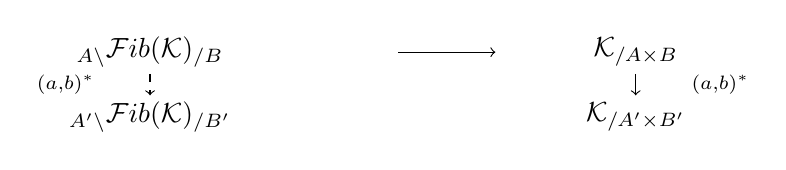
\begin{tikzpicture}[x=1.3em,y=1.3em]
  \node (TL) at (0,1.8) {${}_{A\backslash}\Fib(\mathcal{K})_{/B}$};
  \node (TR) at (13.5,1.8) {$\mathcal{K}_{/A\times B}$};
  \node (BL) at (0,0) {${}_{A'\backslash}\Fib(\mathcal{K})_{/B'}$};
  \node (BR) at (13.5,0) {$\mathcal{K}_{/A'\times B'}$};
  \draw[->] (6.9,1.8) -- (9.6,1.8);
  \draw[->,dashed] (0,1.2) -- (0,0.6);
  \node at (-2.35,0.9) {$\scriptstyle(a,b)^{*}$};
  \draw[->] (13.5,1.2) -- (13.5,0.6);
  \node at (15.85,0.9) {$\scriptstyle(a,b)^{*}$};
\end{tikzpicture}
\end{center}
特别地，一个\trTwoSidedFibration{}的拉回仍是一个\trTwoSidedFibration{}。
\end{proposition}

\begin{proof}
把函子 $(a,b)$ 分解为
$A'\times B'\xrightarrow{\mathrm{id}\times b}A'\times B\xrightarrow{a\times\mathrm{id}}A\times B$，%
可见每次考虑沿一侧作拉回就够了。命题 5.2.4 与练习 5.3.i 证明：沿
$b\colon B'\to B$ 的拉回保持\trCartesianFibration{}与\trCartesianFunctor{}，从而定义出一个%
限制后的函子
\begin{center}
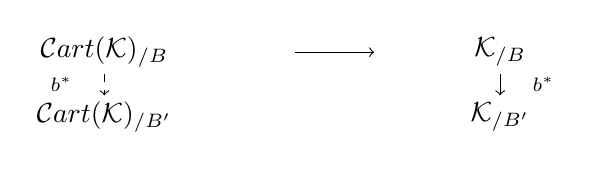
\begin{tikzpicture}[x=1.3em,y=1.3em]
  \node (TL) at (0,1.8) {$\Cart(\mathcal{K})_{/B}$};
  \node (TR) at (11,1.8) {$\mathcal{K}_{/B}$};
  \node (BL) at (0,0) {$\Cart(\mathcal{K})_{/B'}$};
  \node (BR) at (11,0) {$\mathcal{K}_{/B'}$};
  \draw[->] (5.3,1.8) -- (7.5,1.8);
  \draw[->,dashed] (0,1.2) -- (0,0.6);
  \node at (-1.2,0.9) {$\scriptstyle b^{*}$};
  \draw[->] (11,1.2) -- (11,0.6);
  \node at (12.2,0.9) {$\scriptstyle b^{*}$};
\end{tikzpicture}
\end{center}
由于 $\Cart(\mathcal{K})_{/B}$ 中的\trLimit{}与\trIsofibration{}是在
$\mathcal{K}_{/B}$ 中创生的，这一限制后的函子是\trCosmological{}（见引理 10.1.1）。
把这一结果应用于\trInfinityCosmos{} $\coCart(\mathcal{K})_{/A}$ 中的映射
\begin{center}
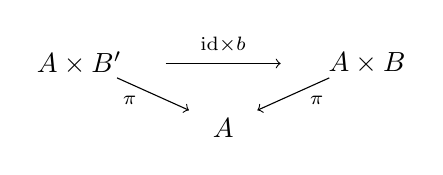
\begin{tikzpicture}[x=1.3em,y=1.3em]
  \node (L) at (0,1.8) {$A\times B'$};
  \node (R) at (8,1.8) {$A\times B$};
  \node (B) at (4,0) {$A$};
  \draw[->] (2.4,1.8) -- (5.6,1.8);
  \node at (4,2.32) {$\scriptstyle\mathrm{id}\times b$};
  \draw[->] (1.05,1.4) -- (3.05,0.5);
  \node at (1.4,0.78) {$\scriptstyle\pi$};
  \draw[->] (6.95,1.4) -- (4.95,0.5);
  \node at (6.6,0.78) {$\scriptstyle\pi$};
\end{tikzpicture}
\end{center}
我们得出：拉回经限制而定义一个\trCosmologicalFunctor
\begin{equation*}
\begin{array}{ccccc}
\Cart(\coCart(\mathcal{K})_{/A})_{/\pi\colon A\times B\to A}
& \hookrightarrow &
(\coCart(\mathcal{K})_{/A})_{/\pi\colon A\times B\to A}
& \hookrightarrow &
\mathcal{K}_{/A\times B}\\[0.5em]
{}_{(\mathrm{id}\times b)^{*}}\dashdownarrow & &
\dashdownarrow_{(\mathrm{id}\times b)^{*}} & &
\downarrow_{(\mathrm{id}\times b)^{*}}\\[0.5em]
\Cart(\coCart(\mathcal{K})_{/A})_{/\pi\colon A\times B'\to A}
& \hookrightarrow &
(\coCart(\mathcal{K})_{/A})_{/\pi\colon A\times B'\to A}
& \hookrightarrow &
\mathcal{K}_{/A\times B'}
\end{array}
\end{equation*}
\end{proof}

\begin{lemma}\label{lem:whiskering-two-sided-fibrations}
若 $A\xleftarrow{q}E\xrightarrow{p}B$ 是从 $A$ 到 $B$ 的一个\trTwoSidedFibration{}，%
$v\colon A\twoheadrightarrow C$ 是一个\trCocartesianFibration{}而
$u\colon B\twoheadrightarrow D$ 是一个\trCartesianFibration{}，那么复合\trSpan
\begin{equation*}
C\xleftarrow{v}A\xleftarrow{q}E\xrightarrow{p}B\xrightarrow{u}D
\end{equation*}
定义一个从 $C$ 到 $D$ 的\trTwoSidedFibration{}。此外，从 $A$ 到 $B$ 的%
\trTwoSidedFibration{}之间的一个\trCartesianFunctor $h$ 诱导出从 $C$ 到 $D$ 的%
\trTwoSidedFibration{}之间的一个\trCartesianFunctor{}：
\begin{center}
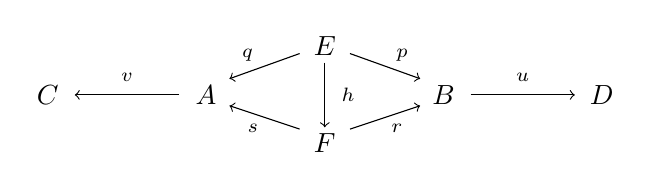
\begin{tikzpicture}[x=1.3em,y=1.3em]
  \node (E) at (3.3,2.7) {$E$};
  \node (A) at (0,1.35) {$A$};
  \node (B) at (6.6,1.35) {$B$};
  \node (C) at (-4.4,1.35) {$C$};
  \node (D) at (11,1.35) {$D$};
  \node (F) at (3.3,0) {$F$};
  \draw[->] (2.6,2.5) -- (0.65,1.8);
  \node at (1.15,2.45) {$\scriptstyle q$};
  \draw[->] (4.0,2.5) -- (5.95,1.8);
  \node at (5.45,2.45) {$\scriptstyle p$};
  \draw[->] (3.3,2.25) -- (3.3,0.45);
  \node at (3.95,1.35) {$\scriptstyle h$};
  \draw[->] (-0.75,1.35) -- (-3.65,1.35);
  \node at (-2.2,1.85) {$\scriptstyle v$};
  \draw[->] (7.35,1.35) -- (10.25,1.35);
  \node at (8.8,1.85) {$\scriptstyle u$};
  \draw[->] (2.6,0.4) -- (0.65,1.05);
  \node at (1.3,0.42) {$\scriptstyle s$};
  \draw[->] (4.0,0.4) -- (5.95,1.05);
  \node at (5.3,0.42) {$\scriptstyle r$};
\end{tikzpicture}
\end{center}
这一\trWhiskering{}复合并不定义一个从 ${}_{A\backslash}\Fib(\mathcal{K})_{/B}$ 到
${}_{C\backslash}\Fib(\mathcal{K})_{/D}$ 的\trCosmologicalFunctor{}，因为由与等价%
纤维化 $v\times u$ 作复合所定义的函子
$(v\times u)_{*}\colon\mathcal{K}_{/A\times B}\to\mathcal{K}_{/C\times D}$
并不保持\trFlexibleWeightedLimit{}（见非例 1.3.6）。
\end{lemma}

\begin{proof}
由定理 7.1.4，逐侧分别考虑复合即可，比如说与一个\trCocartesianFibration{}
$v\colon A\twoheadrightarrow C$ 复合。在\trInfinityCosmos{} $\Cart(\mathcal{K})_{/B}$
中工作，我们手头有\trCocartesianFibration
\begin{center}
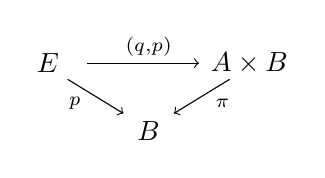
\begin{tikzpicture}[x=1.3em,y=1.3em]
  \node (E) at (0,1.9) {$E$};
  \node (AB) at (5.6,1.9) {$A\times B$};
  \node (B) at (2.8,0) {$B$};
  \draw[->] (1.1,1.9) -- (4.2,1.9);
  \node at (2.8,2.36) {$\scriptstyle(q,p)$};
  \draw[->] (0.55,1.45) -- (2.1,0.5);
  \node at (0.75,0.78) {$\scriptstyle p$};
  \draw[->] (5.05,1.45) -- (3.5,0.5);
  \node at (4.85,0.78) {$\scriptstyle\pi$};
\end{tikzpicture}
\qquad
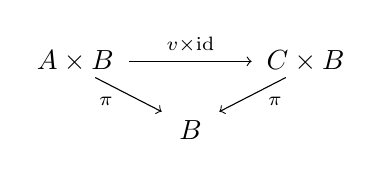
\begin{tikzpicture}[x=1.3em,y=1.3em]
  \node (AB) at (0,1.9) {$A\times B$};
  \node (CB) at (6.4,1.9) {$C\times B$};
  \node (B) at (3.2,0) {$B$};
  \draw[->] (1.5,1.9) -- (4.9,1.9);
  \node at (3.2,2.36) {$\scriptstyle v\times\mathrm{id}$};
  \draw[->] (0.55,1.45) -- (2.4,0.5);
  \node at (0.85,0.78) {$\scriptstyle\pi$};
  \draw[->] (5.85,1.45) -- (4.0,0.5);
  \node at (5.55,0.78) {$\scriptstyle\pi$};
\end{tikzpicture}
\end{center}
它们复合起来定义一个\trCocartesianFibration
\begin{center}
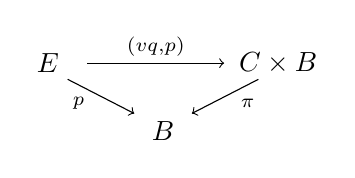
\begin{tikzpicture}[x=1.3em,y=1.3em]
  \node (E) at (0,1.9) {$E$};
  \node (CB) at (6.4,1.9) {$C\times B$};
  \node (B) at (3.2,0) {$B$};
  \draw[->] (1.1,1.9) -- (4.9,1.9);
  \node at (3.0,2.36) {$\scriptstyle(vq,p)$};
  \draw[->] (0.55,1.45) -- (2.4,0.5);
  \node at (0.85,0.78) {$\scriptstyle p$};
  \draw[->] (5.85,1.45) -- (4.0,0.5);
  \node at (5.55,0.78) {$\scriptstyle\pi$};
\end{tikzpicture}
\end{center}
从而如所愿地定义一个从 $C$ 到 $B$ 的\trTwoSidedFibration{}。

由引理 5.2.3，诸 $vq$-\trCocartesian\trCell{}恰是诸 $v$-\trCocartesian\trCell{}的%
$q$-\trCocartesian{}提升。若 $h$ 是从 $q$ 到 $s$ 的一个\trCartesianFunctor{}，那么这些%
\trCell{}显然被保持，这就证明了 $h$ 也定义一个从 $vq$ 到 $vs$ 的\trCartesianFunctor{}。由%
命题 7.1.7(iv)，这就证明了 $h$ 在须化后的\trTwoSidedFibration{}之间定义一个%
\trCartesianFunctor{}。
\end{proof}

\cref{prop:pullback-restricts-two-sided}与\cref{lem:whiskering-two-sided-fibrations}%
结合起来证明：\trTwoSidedFibration{}可以「水平地」复合。

\begin{proposition}\label{prop:horizontal-composite-two-sided}
从 $A$ 到 $B$ 的一个\trTwoSidedFibration{}沿一个从 $B$ 到 $C$ 的%
\trTwoSidedFibration{}的拉回，定义一个从 $A$ 到 $C$ 的\trTwoSidedFibration{}，%
如下列所示：
\begin{center}
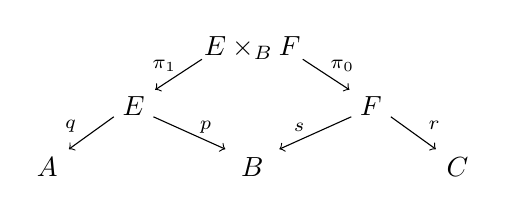
\begin{tikzpicture}[x=1.3em,y=1.3em]
  \node (P) at (3.3,3.3) {$E\times_{B}F$};
  \node (E) at (0,1.7) {$E$};
  \node (F) at (6.6,1.7) {$F$};
  \node (A) at (-2.4,0) {$A$};
  \node (B) at (3.3,0) {$B$};
  \node (C) at (9.0,0) {$C$};
  \draw[->] (1.9,3.0) -- (0.6,2.15);
  \node at (0.85,2.82) {$\scriptstyle\pi_{1}$};
  \draw[->] (4.7,3.0) -- (6.0,2.15);
  \node at (5.8,2.82) {$\scriptstyle\pi_{0}$};
  \draw[->] (-0.55,1.4) -- (-1.8,0.5);
  \node at (-1.75,1.15) {$\scriptstyle q$};
  \draw[->] (0.55,1.4) -- (2.55,0.5);
  \node at (2.0,1.12) {$\scriptstyle p$};
  \draw[->] (6.05,1.4) -- (4.05,0.5);
  \node at (4.6,1.12) {$\scriptstyle s$};
  \draw[->] (7.15,1.4) -- (8.4,0.5);
  \node at (8.35,1.15) {$\scriptstyle r$};
\end{tikzpicture}
\end{center}
\end{proposition}

\begin{proof}
该复合\trTwoSidedFibration{}分两个阶段构造：首先作拉回
\begin{center}
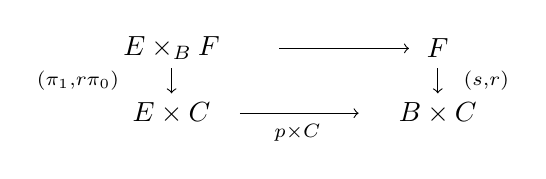
\begin{tikzpicture}[x=1.3em,y=1.3em]
  \node (TL) at (0,1.8) {$E\times_{B}F$};
  \node (TR) at (7.4,1.8) {$F$};
  \node (BL) at (0,0) {$E\times C$};
  \node (BR) at (7.4,0) {$B\times C$};
  \draw[->] (3.0,1.8) -- (6.6,1.8);
  \draw[->] (0,1.25) -- (0,0.55);
  \node at (-2.6,0.9) {$\scriptstyle(\pi_{1},r\pi_{0})$};
  \draw[->] (7.4,1.25) -- (7.4,0.55);
  \node at (8.75,0.9) {$\scriptstyle(s,r)$};
  \draw[->] (1.9,0) -- (5.2,0);
  \node at (3.5,-0.55) {$\scriptstyle p\times C$};
  \node at (1.1,1.1) {$\scriptstyle\lrcorner$};
\end{tikzpicture}
\end{center}
然后将左腿与\trCocartesianFibration{} $q\colon E\twoheadrightarrow A$ 复合。由%
\cref{prop:pullback-restricts-two-sided}与\cref{lem:whiskering-two-sided-fibrations}，%
其结果是一个从 $A$ 到 $C$ 的\trTwoSidedFibration{}。或者，该复合也可以这样构造：%
沿 $A\times s$ 作拉回并与\trCartesianFibration{} $r\colon F\twoheadrightarrow C$
复合，得到另一个从 $A$ 到 $C$ 的\trTwoSidedFibration{}，它与第一个典范同构。
\end{proof}

有了这些结果，我们便可以为我们的例子库增添几个新成员了：

\begin{example}\label{exa:two-sided-fibration-from-cart-cocart}
若 $p\colon E\twoheadrightarrow B$ 是一个\trCartesianFibration{}而
$q\colon F\twoheadrightarrow A$ 是一个\trCocartesianFibration{}，那么由与积投影%
复合而成的\trSpan
\begin{equation*}
A\overset{q}{\twoheadleftarrow}F\overset{\pi}{\twoheadleftarrow}F\times E\overset{\pi}{\twoheadrightarrow}E\overset{p}{\twoheadrightarrow}B
\end{equation*}
依练习 7.1.i 定义一个从 $A$ 到 $B$ 的\trTwoSidedFibration{}。
\end{example}

\begin{example}\label{exa:comma-span-two-sided}
由命题 7.1.6 与\cref{prop:pullback-restricts-two-sided}，一般的逗号\trSpan
\begin{equation*}
C\xleftarrow{p_{1}}\mathrm{Hom}_{A}(f,g)\xrightarrow{p_{0}}B
\end{equation*}
是一个\trTwoSidedFibration{}，因为它是
$A\overset{p_{1}}{\twoheadleftarrow}A^{2}\overset{p_{0}}{\twoheadrightarrow}A$
的一个\trPullback{}。
\end{example}

\begin{example}\label{exa:horizontal-composite-comma-spans}
由\cref{prop:horizontal-composite-two-sided}与\cref{exa:comma-span-two-sided}，%
逗号\trSpan{}的水平复合也是\trTwoSidedFibration{}。例如，\trTwoSidedFibration
\begin{equation*}
A\overset{p_{1}}{\twoheadleftarrow}A^{2}
\overset{p_{n+1}}{\twoheadleftarrow}A^{n+1}
\overset{p_{0}}{\twoheadrightarrow}A
\end{equation*}
是箭头\trSpan{}
$A\overset{p_{1}}{\twoheadleftarrow}A^{2}\overset{p_{0}}{\twoheadrightarrow}A$
的 $n$ 元水平复合。
\end{example}

其他值得注意的\trTwoSidedFibration{}还包括逗号\trSpan{}的水平复合，其特例之一%
将在下一节中占据显要地位。
